\documentclass[a4paper,12pt,twoside,UTF8,hyperref]{ctexart}
\usepackage{times}%全文英文字体使用Times New Roman;
\linespread{1.5}%全文1.5倍行距;
%========================电子文档与超链接======================
\usepackage[pdftex,linkcolor=blue,citecolor=blue,backref=page,hyperfootnotes=false]{hyperref}
\usepackage[a4paper,left=3.0cm,right=2.0cm,top=3.51cm,bottom=4.25cm]{geometry}
\hypersetup{
 colorlinks = true,
 linkcolor=blue,
 bookmarks = true,
 bookmarksopen = true,
 pdfborder=0 0 0,
 hyperfootnotes=false,
 %pdfpagemode = FullScreen,
 pdfstartview = Fit,
 pdftitle = {中南大学本科毕业论文LaTeX模板},
 pdfauthor = {Chai Xingtao}
}
\pdfbookmark[1]{Contents}{contents}
%===============================================================

%=========================设=置=页=眉===========================
\usepackage{fancyhdr}% 为了保证正确长度的页眉下划线,fancyhdr宏包要在geometry宏包后使用;
\pagestyle{fancy}
\fancyhf{}
\lhead{
\includegraphics[scale=0.13]{./pictures/CSU_Logo.jpg}}
\usepackage{lastpage}
\rhead{\small\heiti 中南大学本科毕业论文\,\LaTeX\,模板说明}
%===============================================================

%==========================章节格式=============================
\usepackage{titlesec}
\titleformat{\section}[hang]{\Large\bfseries\center}{第\,\thesection\,章 \quad}{0pt}{}{}
\titleformat{\subsection}[hang]{\normalsize\bfseries\raggedright}{\thesubsection\quad}{0pt}{}{}
\titleformat{\subsubsection}[hang]{\normalsize\kaishu\raggedright}{\thesubsubsection\quad}{0pt}{}{}
\titlespacing*{\section}{0pt}{0pt}{19.2pt}[0pt]
\titlespacing*{\subsection}{0pt}{0pt}{0pt}[0pt]
\titlespacing*{\subsubsection}{0pt}{0pt}{0pt}[0pt]
%===============================================================

%============================目录===============================
\usepackage{titletoc}
\titlecontents{section}[0mm]{}{}{}{}[]
\dottedcontents{section}[0.0em]{\normalsize}{1.0em}{4pt}
\dottedcontents{subsection}[3.0em]{\normalsize}{2.0em}{4pt}
\dottedcontents{subsubsection}[6.0em]{\normalsize}{3.0em}{4pt}
%===============================================================

%==========================脚注格式=============================
\usepackage{pifont}%更好看的一个脚注格式
\renewcommand\thefootnote{\ding{\numexpr171+\value{footnote}}}% 更好看的一个脚注格式
\usepackage[perpage]{footmisc}%脚注每页清零编号
%===============================================================

%==========================插入图片=============================
\usepackage{graphicx}
\usepackage{subfigure}%两图并排
\usepackage{picinpar}%文字绕排
\usepackage{caption}
\captionsetup{font=small,labelfont=bf,labelsep=quad}
\captionsetup{skip=0pt}%标题与浮动环境内容的垂直间距无额外间距(设置为0pt);
%===============================================================

%==========================插入表格=============================
\usepackage{booktabs,multirow}%三线表
\usepackage{longtable}%长表格
\usepackage{bigstrut}
\usepackage{diagbox}
\usepackage{makecell}
\usepackage{tabularx}
\newcolumntype{Y}{>{\centering\arraybackslash}X}
%==========================解决三线表竖线过短的问题=============================
\renewcommand{\cmidrulesep}{0mm} %定义两条相邻\cmidrule之间的间隔
\setlength{\aboverulesep}{0mm} %在线条[不包括\toprule]上面增加一段垂直距离,此处为0mm
\setlength{\belowrulesep}{0mm} %在线条[不包括\bottomrule]下面增加一条垂直距离,此处为0mm
\setlength{\abovetopsep}{0cm}  %在线条\toprule上面,即表格与上面的文字之间的距离。
\setlength{\belowbottomsep}{0cm}%在线条\bottomrule下面,即表格与下面的文字之间的距离。
%===============================================================

%==========================数学公式=============================
\usepackage{amsmath}%公式
\usepackage{amssymb}
\usepackage{bm}%粗体
\usepackage{upgreek}%直立希腊字母
\usepackage{mhchem}%化学公式 \ce{SiO2} 或 \ce{H2O}
\DeclareMathOperator\dif{d\!}%微分算子\frac{\dif y}{dif x}
%\usepackage{xfrac}%行内小分式
\newenvironment{sequation}{\begin{equation}\small}{\end{equation}}
\newenvironment{tequation}{\begin{equation}\tiny}{\end{equation}}
%===============================================================

%==========================程序代码=============================
\usepackage{listings}
%===============================================================

%==========================使用彩色=============================
%\usepackage[usenames,dvipsnames]{color}
\usepackage{color}
\usepackage[table]{xcolor}
\usepackage{colortbl}
\definecolor{mygray}{gray}{.9}
\definecolor{mypink}{rgb}{.99,.91,.95}
\definecolor{mycyan}{cmyk}{.3,0,0,0}
%================================================================

%=============================其它===============================
\usepackage{siunitx}%摄氏度 \SI{100}{\degreeCelsius}
\makeatletter%罗马数字
\newcommand{\rmnum}[1]{\romannumeral #1}% 罗马数字
\newcommand{\Rmnum}[1]{\expandafter\@slowromancap\romannumeral #1@}%罗马数字
\makeatother%罗马数字 \Rmnum{1} 或 \Rmnum{2} 或 \rmnum{3}
\usepackage{xfrac}%行内小分式
%==================================================================

%=============================文献格式===============================
\usepackage{gbt7714}%文献格式使用GB/T7714-2015标准;
\newcommand{\upcite}[1]{\textsuperscript{\textsuperscript{\cite{#1}}}}
\usepackage{natbib}
\renewcommand\bibfont{\small\kaishu}%文献字体改用5号字体;
\setlength\bibsep{0pt}%取消不同文献条目之间的距离;
\usepackage{url}
%==================================================================

%=========================一个更好的下划线设置=======================
\usepackage{ulem}

\usepackage{enumitem}

\usepackage{hhline}% 双线表

\newcommand\dlmu[2][4cm]{\hskip1pt\underline{\hb@xt@ #1{\hss#2\hss}}\hskip3pt}

%=========================公式按章编号===============================
\makeatletter
\@addtoreset{equation}{section}
\makeatother
\renewcommand{\theequation}{\arabic{section}-\arabic{equation}}

\makeatletter
\@addtoreset{figure}{section}
\makeatother
\renewcommand{\thefigure}{\thesection\,-\,\arabic{figure}}

\makeatletter
\@addtoreset{table}{section}
\makeatother
\renewcommand{\thetable}{\thesection\,-\,\arabic{table}}
%==================================================================

\usepackage{ifpdf}

\newtheorem{thm}{定理}

%==============积分符号修改,改原倾斜的积分符号为直立体==================
\usepackage{amsmath,amssymb}
\DeclareSymbolFont{EulerExtension}{U}{euex}{m}{n}
\DeclareMathSymbol{\euintop}{\mathop} {EulerExtension}{"52}
\DeclareMathSymbol{\euointop}{\mathop} {EulerExtension}{"48}
\let\intop\euintop
\let\ointop\euointop
%==================================================================

\usepackage{doc}%BibTeX显示;
\begin{document}
\begin{titlepage}
\phantom{\LARGE 中南大学}
\begin{figure}[htbp]
  \centering
  % Requires \usepackage{graphicx}
  
\includegraphics[scale=0.45]{./pictures/CSU_Logo.jpg}\\
\end{figure}

\phantom{中南大学}

\begin{center}
{\fontsize{45pt}{14.4pt}\heiti 本科毕业设计(论文)}
\end{center}

\begin{center}
 {\zihao{1}\rmfamily GRADUATION DESIGN (THSIS)}
\end{center}

\phantom{中南大学}

\phantom{中南大学}

\begin{table}[htbp]
\centering
\LARGE\kaishu
\begin{tabular}{cc}
  {\heiti 题\qquad 目:} & \makecell{中南大学本科毕业论文\\ \,\LaTeX\,模板说明} \\
  \cline{2-2}
  {\heiti 学生姓名:} &  $XXX$\\
  \cline{2-2}
  {\heiti 指导老师:} & $XXX$ \\
  \cline{2-2}
  {\heiti 学\qquad 院:} & $XXX$ \\
  \cline{2-2}
  {\heiti 专业班级:} & $XXX$ \\
  \cline{2-2}
\end{tabular}
\end{table}
\vspace{32pt}
\begin{center}
\zihao{2}{\heiti 非本科生院制}\\

\zihao{-2}{\heiti 2019年12月}

\end{center}
\end{titlepage}


\clearpage
\phantom{s}
\thispagestyle{empty}
\newpage

\setcounter{page}{1}
\pagenumbering{Roman}
\cfoot{\small\thepage}
\vspace*{-21.6pt}
\begin{center}
\zihao{-2}\heiti
中南大学本科毕业论文\,\LaTeX\,模板说明
\end{center}
\par
\begin{center}
\zihao{3}\heiti
\phantomsection
\addcontentsline{toc}{section}{摘要}
摘要
\end{center}

\par
本项目为年产\,50\,万吨MTO工厂的初步设计。通过分析当前国内外MTO生产和研究现状,对生产工艺进行了选择论证。然后运用Aspen软件模拟初步的工艺流程,并通过对一系列工艺参数,如精馏塔的塔板数—产品纯度、进料塔板数—产品纯度、产品纯度—回流比、再沸器负荷—回流比等进行灵敏度分析,优化设备操作条件,提高工艺的合理性和经济性。本设计还针对工艺流程进行换热网络设计和对全局换热网络进行了优化和评估,通过内部流股之间相互换热以减少公用工程的消耗,最终优化后节约$\,79.4\%\,$的热公用工程资源和$\,73.7\%\,$的冷公用工程资源。本设计还运用水夹点技术优化了用水网络,根据水硬度分类处理水操作单元,并合理再生利用,使得本项目新鲜水用量和废水排放量达到最小,优化后的用水网络节约用水$\,53.59\%\,$。本设计对于MTO工厂的生产和设计建造具有一定的现实指导意义。

\bigskip
\noindent\textbf{关键字:}工厂\quad 设计\quad MTO\quad 工艺\quad 水夹点\quad  网络\quad  控制

\newpage
\vspace*{-21.6pt}
\begin{center}
\zihao{-2}\bfseries
\rmfamily Description of \LaTeX\,template for the undergraduate thesis of Central South University
\end{center}
\par
\phantomsection
\addcontentsline{toc}{section}{ABSTRACT}
\begin{center}
\zihao{3}\rmfamily\bfseries
ABSTRACT
\end{center}

\par
This project is the preliminary design of a MTO plant with an annual output of 500,000 tons of light olefins. Based on the current production and research situation all through the world, the production method was selected and demonstrated. Aspen software was used to simulate the preliminary process. Heat integration method was applied to optimize the heat exchange network. Rational heat exchange between process streams were suggested which resulted in the decreasing of utilities consumption and exchanger number. The heat integration leaded to energy saving of $79.4\%$ of heat utilities and $73.7\%$ of the cold utilities. In addition, the water pinch technology was also implemented to optimize the water network. The water operating unit was classified according to water hardness, with a reasonable recycling. The amount of fresh water consumption and wastewater emission was minimized. The optimized water network achieved $53.59\%$ water saving. Finally, a preliminary economic analysis to the entire project was estimated in order to get the project construction cost and profitability. In summary, this design is of some practical significance for the production and design of the MTO industry.

\bigskip
\noindent\textbf{Key Words:}\quad Plant design\quad Sensitivity analysis\quad Energy balance calculation\quad Water pinch\quad Dynamic control

\newpage

\phantomsection%设置“幻影标题”,解决额外插入目录(\addcontentsline)后总是引用到第一页的问题;
\addcontentsline{toc}{section}{目录}
\vspace*{-21.6pt}
\tableofcontents
\newpage

\setcounter{page}{1}
\pagenumbering{arabic}
\cfoot{\small 第\,\thepage\,页\quad 共\,\pageref{LastPage}\,页}
\newpage\vspace*{-21.6pt}
\section{绪论}%每一个一级标题(\section)单独起页;
\subsection{写给读者}
本\LaTeX 模板格式完全参考原Word模板“附件7:中南大学毕业设计(论文)模板.docx”,是由作者(本科学生)自己编写的\LaTeX 模板,不是官方书写的模板。

本\LaTeX 模板适用于对\LaTeX 具有一定程度了解的读者,对新手可能不友好:对\LaTeX 各类环境命令不熟悉,或在编译过程中出现的问题不能及时解决,其排版效率将远不如Word。作者认为,读者至少已经看完了流行的入门教程《112分钟学会\LaTeX 》。

\subsection{\LaTeX 与Word的比较}
先写在前面,就作者长期作用\LaTeX 和Word 进行科技论文或一般文章的书写排版的经验来看:作为文字书写和排版工具,综合来看,\textcolor{red}{Word 或WPS 是要强于\LaTeX 的}。

\subsubsection{\LaTeX 的特点}
\LaTeX 是一种基于\TeX 的文档排版系统,为减轻写作、排版一肩挑的负担,将大片排版的格式细节隐藏在若干样式之后,是现在最流行的科技写作——尤其是数学写作的工具之一。

相比Word,在公式编辑的格式控制、公式编辑的易用程度与编辑效率(包括作者,在Word中编辑公式时,仍然使用MathType中的\TeX 输入方式)、交叉引用、文献管理上,\LaTeX 要比Word 好用太多,可以说是全面胜出,所以学术圈更青睐于\LaTeX 。

漂亮。不少文字排版工作者都认为用\LaTeX 书写出来的文章要比Word好看很多。

在有现成模板的情况下,\LaTeX 模板用起来比Word模板更方便。

\LaTeX 系统是免费的,而Word和MathType是商业软件,对于大部分人而言(至少本科生),收费高昂。

\subsubsection{Word的特点}
但Word的优点在诸多方面远远胜于\LaTeX :

简单,易上手。Word除了书写正文需要敲敲键盘,排版可能只需要点一点鼠标。由于“所见即所得”,Word上手难度极小,简单易懂。而\LaTeX 具有大量让人望而生畏的代码,有烦人的debug,如果只学习了部分\LaTeX 环境命令的知识,可能难以排版出一篇合格的文章。

Word本身有文字编辑上的辅助功能,而一般\LaTeX 编辑器只有代码书写辅助功能(还很鸡肋),对于大段纯文字的写作,完全没必要使用\LaTeX 。

Word在表格上编辑排版略胜于\LaTeX 。

\subsection{本章小节}
刘海洋老师在《\LaTeX 入门》一书中写到:“\LaTeX 是一种并不简单的计算机语言,不能只点点鼠标就弄好一篇漂亮的文章,也不是一两个小时的泛泛了解就尽能对付得过去。”

对于元素众多,格式复杂的文章,\LaTeX 可能更胜Word一筹,但对于大部分时间遇到的文章,Word远优于\LaTeX 。

本\LaTeX 模板可运用CTeX+WinEdt 或CTeX+TeXstudio进行编译和编辑。

\newpage\vspace*{-21.6pt}
\section{组织你的文本}
从本章开始,对论文中可能出现的各类\,\LaTeX 环境与命令进行说明,主要包括文字与符号、论文的结构层次、图表的绘制、自动化工具(目录格式与文献格式)进行说明。

\subsection{文字与说明}
正文中文使用小四宋体,英文使用Times New Roman字体。其余特殊环境字体大小在后文中说明。

行距为word中的1.5倍行距,总行距为$1.5\times 1.2\times 12\mathrm{pt} $。

\subsection{段落与文本环境}
\subsubsection{列表环境}
文中可以使用列表:
\begin{enumerate}
  \item 中文
  \item 英语
  \item 法语
\end{enumerate}

也可以使用下列更常用和紧凑的一个定制格式:
\begin{enumerate}[itemsep=0pt,parsep=0pt,label=(\arabic*)]
  \item 中文
  \item 英语
  \item 法语
\end{enumerate}

\subsubsection{脚注环境}
在正文中可以使用脚注进行文字说明,同时对原\LaTeX 中默认的脚注编号格式进行了优化,例如\footnote{这是一个更好的带圆圈的脚注}。

\subsubsection{程序代码环境}
当你的论文中有程序代码需要列出时,可以使用作者为你定制的程序代码环境,见附录。当然,这里只对Matlab语言进行了设置,对于其它常见语言(C++、Python等),读者可以自行进行关键字高亮、字体大小等进行设置。

\textcolor{red}{注意:在排版程序时,如果您的程序中包含中文字符,请使用规避符“}\verb"` `"\textcolor{red}{”:}

\verb"n=2000;%`投针次数figure;`"

\subsection{文档的结构层次}
与原Word版的文档结构层次相同,划分为章、节和小节三部分。读者只需分别在\verb"\section{}"、\verb"\subsection{}"和\verb"\subsubsection{}"中填入标题即可,如\\
\verb"\section{概论}"产生“第1章\quad 概论”,无需加“第1章”字样。

\textcolor{red}{注意,由于一级标题要求另起一页开始且分行,所以应在}\verb"\section{}"\textcolor{red}{命令前加}\verb"\newpage\vspace*{-21.6pt}"\textcolor{red}{命令。}

$21.6\mathrm{pt}$\,是小四字体($12\mathrm{pt}$)的1.5倍行距:$12\mathrm{pt}\times 1.2\times 1.5 = 21.6\mathrm{pt}$。

三层标题的字体大小及缩进与原Word模板无异。读者无需更改。

\subsection{页面格式设计}
\subsubsection{页边距}
左页边距为$3.0\mathrm{cm}$、右页边距为$2.0\mathrm{cm}$,且全文使用双面打印格式(\verb"twoside"),即单页左3右2,双页左2右3,修复了原Word模板中双面打印左右边距错误,不便装订的问题。

由于\LaTeX 与Word中计算上下页边距的方式不同(\LaTeX 上下边距包含了页眉页脚,而Word相反),故在\LaTeX 中将页眉页脚的距离计算了进来。

最终导言区geometry宏包中的页边距命令为:

\verb"a4paper,left=3.0cm,right=2.0cm,top=3.51cm,bottom=4.25cm"

\subsubsection{页眉和页脚}
页眉和页脚的格式与原Word模板相同。同时作者默认只有“摘要”、“ABSTRACT”和“目录”三部分使用罗马字体页码。

\newpage\vspace*{-21.6pt}
\section{自动化工具}
\subsection{目录格式}
目录格式在原Word模板格式的基础上额外添加了“摘要”、“ABSTRACT”和“目录”三部分,如不需要,则将“THSIS\_csu.tex”或“abstract.tex”文件中的

\verb"\phantomsection"

\verb"\addcontentsline{toc}{section}{摘要}"

等命令注释掉或删除。

本\LaTeX 模板与原Word模板中的目录各级标题的字体与缩进无异,但一级标题不是“第1章\quad 概论”,而是“1\quad 概论”,因为作者未能在titletoc宏包中找到类似设置,读者如有能力,请自行设置。

本模板中导言区titletoc宏包的设置命令如下:

\verb"\usepackage{titletoc}"

\verb"\titlecontents{section}[0mm]{}{}{}{}[]"

\verb"\dottedcontents{section}[0.0em]{\normalsize}{1.0em}{4pt}"

\verb"\dottedcontents{subsection}[3.0em]{\normalsize}{2.0em}{4pt}"

\verb"\dottedcontents{subsubsection}[6.0em]{\normalsize}{3.0em}{4pt}"

\subsection{交叉引用}
本模板生成的pdf文件中包含书签,方便电子档阅读,如使用SumatraPDF:“查看”$\to$“书签”。

目录、图表的标题、文献引用和URL地址都添加了彩色超链接功能,对于目录、图表的标题和文献引用为蓝色,而URL地址为洋红色。

其中,文献引用中:在正文中点击文献引用编号“[1]”,可链接至该条参考文献,在该条参考文献后有另一超链接,为该条文献引用的位置页码,例\cite{Meta_CN}。

如希望采用黑色超链接(特别是需要打印时),请在导言区hyperrdf宏包设置中更改\,\verb"colorlinks = true"为\,\verb"colorlink = false"。

同时在hyperrdf宏包设置中更改以下内容:

\verb"pdftitle = {中南大学本科毕业论文LaTeX模板},"

\verb"pdfauthor = {Chai Xingtao}"

上述两条为生成的PDF文档属性。

\subsection{文献格式}
文献格式采用国家标准GB/T 7714-2015格式,格式宏包和格式文件见\\
“gbt7714.sty”、“gbt7714-plain.bst”和“gbt7714-unsrt.bst”。

本模板使用\LaTeX 常用的\BibTeX 进行文献管理。

\newpage\vspace*{-21.6pt}
\section{图表的绘制}
\subsection{公式格式}
本\LaTeX 模板中的公式字体和大小、公式编号与原Word模板无异。例如:

对于三维、瞬态、可压缩牛顿流体的流动与传热现象,其守恒控制方程见如下:

质量守恒方程见式\,(\ref{equ:zhiLiang})。

\begin{equation}\label{equ:zhiLiang}
\frac{\partial\rho}{\partial t}+div\left(\rho u\right)=0
\end{equation}

$X$、$Y$和$Z$方向动量守恒方程分别见式\,(\ref{equ:dongLiangX})、式\,(\ref{equ:dongLiangY})和式\,(\ref{equ:dongLiangZ})。

\begin{equation}\label{equ:dongLiangX}
\frac{\partial\left(\rho u\right)}{\partial t} + div\left(\rho uu\right)=div\left(\mu\mathrm{grad}u\right)-\frac{\partial P}{\partial x}+S_u
\end{equation}

\begin{equation}\label{equ:dongLiangY}
\frac{\partial\left(\rho v\right)}{\partial t} + div\left(\rho vu\right)=div\left(\mu\mathrm{grad}v\right)-\frac{\partial P}{\partial y}+S_v
\end{equation}

\begin{equation}\label{equ:dongLiangZ}
\frac{\partial\left(\rho w\right)}{\partial t} + div\left(\rho wu\right)=div\left(\mu\mathrm{grad}w\right)-\frac{\partial P}{\partial z}+S_w
\end{equation}

能量守恒方程见式\,(\ref{equ:nengLiang})。
\begin{equation}\label{equ:nengLiang}
\frac{\partial\left(\rho T\right)}{\partial t}+div\left(\rho uT\right)=div\left(\frac{k}{c}\mathrm{grad}T\right)+S_T
\end{equation}

另,积分符号进行了优化,在原amsmath宏包中倾斜积分符号更改为了直立体:

\begin{equation}\label{equ:int}
  \int_0^{2\uppi}\sin x = 0
\end{equation}

\subsection{表格格式}

正文中所有表格均采用三线表,例如表\,(\ref{tab:test1})。为文章紧凑,所有表格均采用浮动体。

\textcolor{red}{注意:在浮动体中应更改字体大小,添加}\verb"\small"\textcolor{red}{命令,在}\verb"\caption{}"\textcolor{red}{中添加命令}\verb"\heiti "\textcolor{red}{命令。}

\begin{table}[htbp]
\small
  \centering
  \caption{\heiti 森林生态系统服务价值的敏感系数}\label{tab:test1}
    \begin{tabularx}{\textwidth}{cYYY}
    \toprule
    \phantom{year}Year\phantom{year}  & $CIF_f$  & $CIF_p$  & $CIF_g$ \\
    \midrule
    2006  & 7.4   & 2.59  & 0.07 \\
    2007  & 2.54  & 19.32 & 0.48 \\
    2008  & 6.07  & 12.78 & 11.56 \\
    2009  & 1.78  & 20.14 & 0.38 \\
    2010  & 1.32  & 0.61  & 0.12 \\
    2011  & 1.64  & 2.9   & 0.2 \\
    2012  & 1.02  & 12.57 & 1.38 \\
    \bottomrule
    \end{tabularx}
\end{table}

当表中行数较多,可以使用表格间隔底纹,见表\,(\ref{tab:test2})。
\begin{table}[htbp]
\small
  \centering
  \caption{\heiti 森林生态系统服务价值的敏感系数}\label{tab:test2}
    \begin{tabularx}{\textwidth}{cYYY}
    \toprule
    \phantom{year}Year\phantom{year}  & $CIF_f$  & $CIF_p$  & $CIF_g$ \\
    \midrule
    2006  & 7.4   & 2.59  & 0.07 \\
        \rowcolor{mygray}
    2007  & 2.54  & 19.32 & 0.48 \\
    2008  & 6.07  & 12.78 & 11.56 \\
        \rowcolor{mygray}
    2009  & 1.78  & 20.14 & 0.38 \\
    2010  & 1.32  & 0.61  & 0.12 \\
        \rowcolor{mygray}
    2011  & 1.64  & 2.9   & 0.2 \\
    2012  & 1.02  & 12.57 & 1.38 \\
    \bottomrule
    \end{tabularx}
\end{table}

另书写论文中常用的几个表格格式,见表\,(\ref{tab:ZhuChengFenJieGuo})、表\,(\ref{tab:PaiMIng})和表\,(\ref{tab:yi})

\begin{table}[htbp]
\footnotesize
  \centering
  \caption{\heiti 主成分分析结果}\label{tab:ZhuChengFenJieGuo}
  \begin{tabularx}{\textwidth}{cYYY||cYYY}
    \toprule
    % after \\: \hline or \cline{col1-col2} \cline{col3-col4} ...
    序号 & 特征根 & 贡献率 & \multicolumn{1}{c||}{累积贡献率} & 序号 & 特征根 & 贡献率 & 累积贡献率 \\
    \hhline{----||----}
    1 & 6.2865 & 48.3575  & 48.3575 & 8 & 0.1067 & 0.8210 &  98.8545 \\
    2 & 2.7959 & 21.5067 & 69.8642 & 9 & 0.0663 & 0.5102 &  99.3647 \\
    3 & 2.0499 & 15.7685 & 85.6327 & 10 & 0.0509 & 0.3914 & 99.7561 \\
    4 & 0.7560 & 5.8152 & 91.4479 & 11 & 0.0136 & 0.1044 & 99.8605 \\
    5 & 0.3919 & 3.0146 & 94.4625 & 12 & 0.0106 & 0.0813 & 99.9418 \\
    6 & 0.2543 & 1.9564 & 96.4188 & 13 & 0.0076 & 0.0582 & 100.0000 \\
    7 & 0.2099 & 1.6146 & 98.0335 &   &   &   &   \\
    \bottomrule
  \end{tabularx}
\end{table}

\begin{table}[htbp]
\footnotesize
  \centering
  \caption{\heiti 排名和综合结果}\label{tab:PaiMIng}
  \begin{tabular}{ccccccccc}
    \toprule
    % after \\: \hline or \cline{col1-col2} \cline{col3-col4} ...
    地区 & 广东 & 江苏 & 山西 & 浙江 & 河南 & 湖南 & 上海 & 湖北 \\
    \midrule
    名次 & 1 & 2 & 3 & 4 & 5 & 6 & 7 & 8 \\
    综合评价值 & \phantom{-}3.1511  &  \phantom{-}3.0754 &   \phantom{-}2.1268 &   \phantom{-}1.7027  &  \phantom{-}0.7627 &   \phantom{-}0.6234 &   \phantom{-}0.4570  &  \phantom{-}0.4079 \\
    \bottomrule
  \end{tabular}
  \begin{tabular}{ccccccccc}
    \toprule
    % after \\: \hline or \cline{col1-col2} \cline{col3-col4} ...
    地区 & 河北 & 北京 & 四川 & 安徽 & 辽宁 & 福建 & 天津 & 江西 \\
    \midrule
    名次 & 9 & 10 & 11 & 12 & 13 & 14 & 15 & 16 \\
    综合评价值 & \phantom{-}0.3821  &  \phantom{-}0.3371 &   \phantom{-}0.3144  &  \phantom{-}0.2034 &   \phantom{-}0.1928  &  \phantom{-}0.1223  &  \phantom{-}0.1004  &  -0.2223  \\
    \bottomrule
  \end{tabular}
  \begin{tabular}{ccccccccc}
    \toprule
    % after \\: \hline or \cline{col1-col2} \cline{col3-col4} ...
    地区 & 重庆 & 陕西 & 吉林 & 黑龙江 & 广西 & 山西 & 内蒙古 & 云南 \\
    \midrule
    名次 & 17 & 18 & 19 & 20 & 21 & 22 & 23 & 24 \\
    综合评价值 & -0.2520  & -0.2621 &  -0.2750  & -0.3306 &  -0.3431 &  -0.4451  & -0.5312 &  -0.8562  \\
    \bottomrule
  \end{tabular}
  \begin{tabular}{ccccccccc}
    \toprule
    % after \\: \hline or \cline{col1-col2} \cline{col3-col4} ...
    地区 & 新疆 & 贵州 & 宁夏 & 海南 & 甘肃 & 青海 & 西藏 &  \\
    \midrule
    名次 & 25 & 26 & 27 & 28 & 29 & 30 & 31 &  \\
    综合评价值 & -0.8786  & -1.0786 &  -1.1792 &  -1.1870 &  -1.2515 &  -1.6782 &  -3.1887 &\phantom{-0.0000}\\
    \bottomrule
  \end{tabular}
\end{table}

\begin{table}[htbp]
  \centering
  \small
    \caption{\heiti 伊拉克与中国的各个因素的贡献率}\label{tab:yi}
    \begin{tabular}{cccccc}
    \toprule
    国家 &  & \multicolumn{2}{c}{伊拉克} & \multicolumn{2}{c}{中国}\\
    \midrule
    一级指标 & 二级指标  & 权重    & 贡献率   & 权重    & 贡献率 \\
    \midrule
    \multirow{3}*{经济} & 人均GDP & \multirow{3}*{38\%} & 20.32\% & \multirow{3}*{40\%} & 24.2\% \\
    \cmidrule{2-2}\cmidrule{4-4}\cmidrule{6-6}
          & \multicolumn{1}{c}{国民收入} &       & 9.41\%  &       & 10.23\% \\
    \cmidrule{2-2}\cmidrule{4-4}\cmidrule{6-6}
          & \multicolumn{1}{c}{失业率} &       & 9.27\%  &       & 2.57\% \\
    \midrule
    \multirow{3}*{社会} & 人口密度  & \multirow{3}*{22\%} & 13.24\% & \multirow{3}*{17\%} & 11.87\% \\
    \cmidrule{2-2}\cmidrule{4-4}\cmidrule{6-6}
          & 获得改善水源人口所占的百分比 &       & 4.45\%  &       & 2.34\% \\
          \cmidrule{2-2}\cmidrule{4-4}\cmidrule{6-6}
          & 公共医疗卫生支出所占GDP 的百分比 &       & 4.31\%  &       & 2.79\% \\
    \midrule
    \multirow{3}*{政治} & 军费支出所占GDP百分比 & \multirow{3}*{29\%} & 17.45\% & \multirow{3}*{25\%} & 11.21\% \\
    \cmidrule{2-2}\cmidrule{4-4}\cmidrule{6-6}
          & 武装部队人员总数 &       & 6.34\%  &       & 12.34\% \\
          \cmidrule{2-2}\cmidrule{4-4}\cmidrule{6-6}
          & 国际谋杀犯罪率 &       & 3.21\%  &       & 1.45\% \\
    \midrule
    \multirow{3}*{生态} & 人均碳排放量 & \multirow{3}*{11\%} & 1.97\%  & \multirow{3}*{18\%} & 5.87\% \\
    \cmidrule{2-2}\cmidrule{4-4}\cmidrule{6-6}
          & 年均气温  &       & 3.23\%  &       & 2.45\% \\
          \cmidrule{2-2}\cmidrule{4-4}\cmidrule{6-6}
          & 年降水量  &       & 5.8\%   &       & 2.68\% \\
    \bottomrule
    \end{tabular}
\end{table}%

\subsection{图片格式}
图片也采用浮动体,以使文章紧凑,见图\,(\ref{fig:dynamic})。

\begin{figure}[htbp]
  \centering
  % Requires \usepackage{graphicx}
  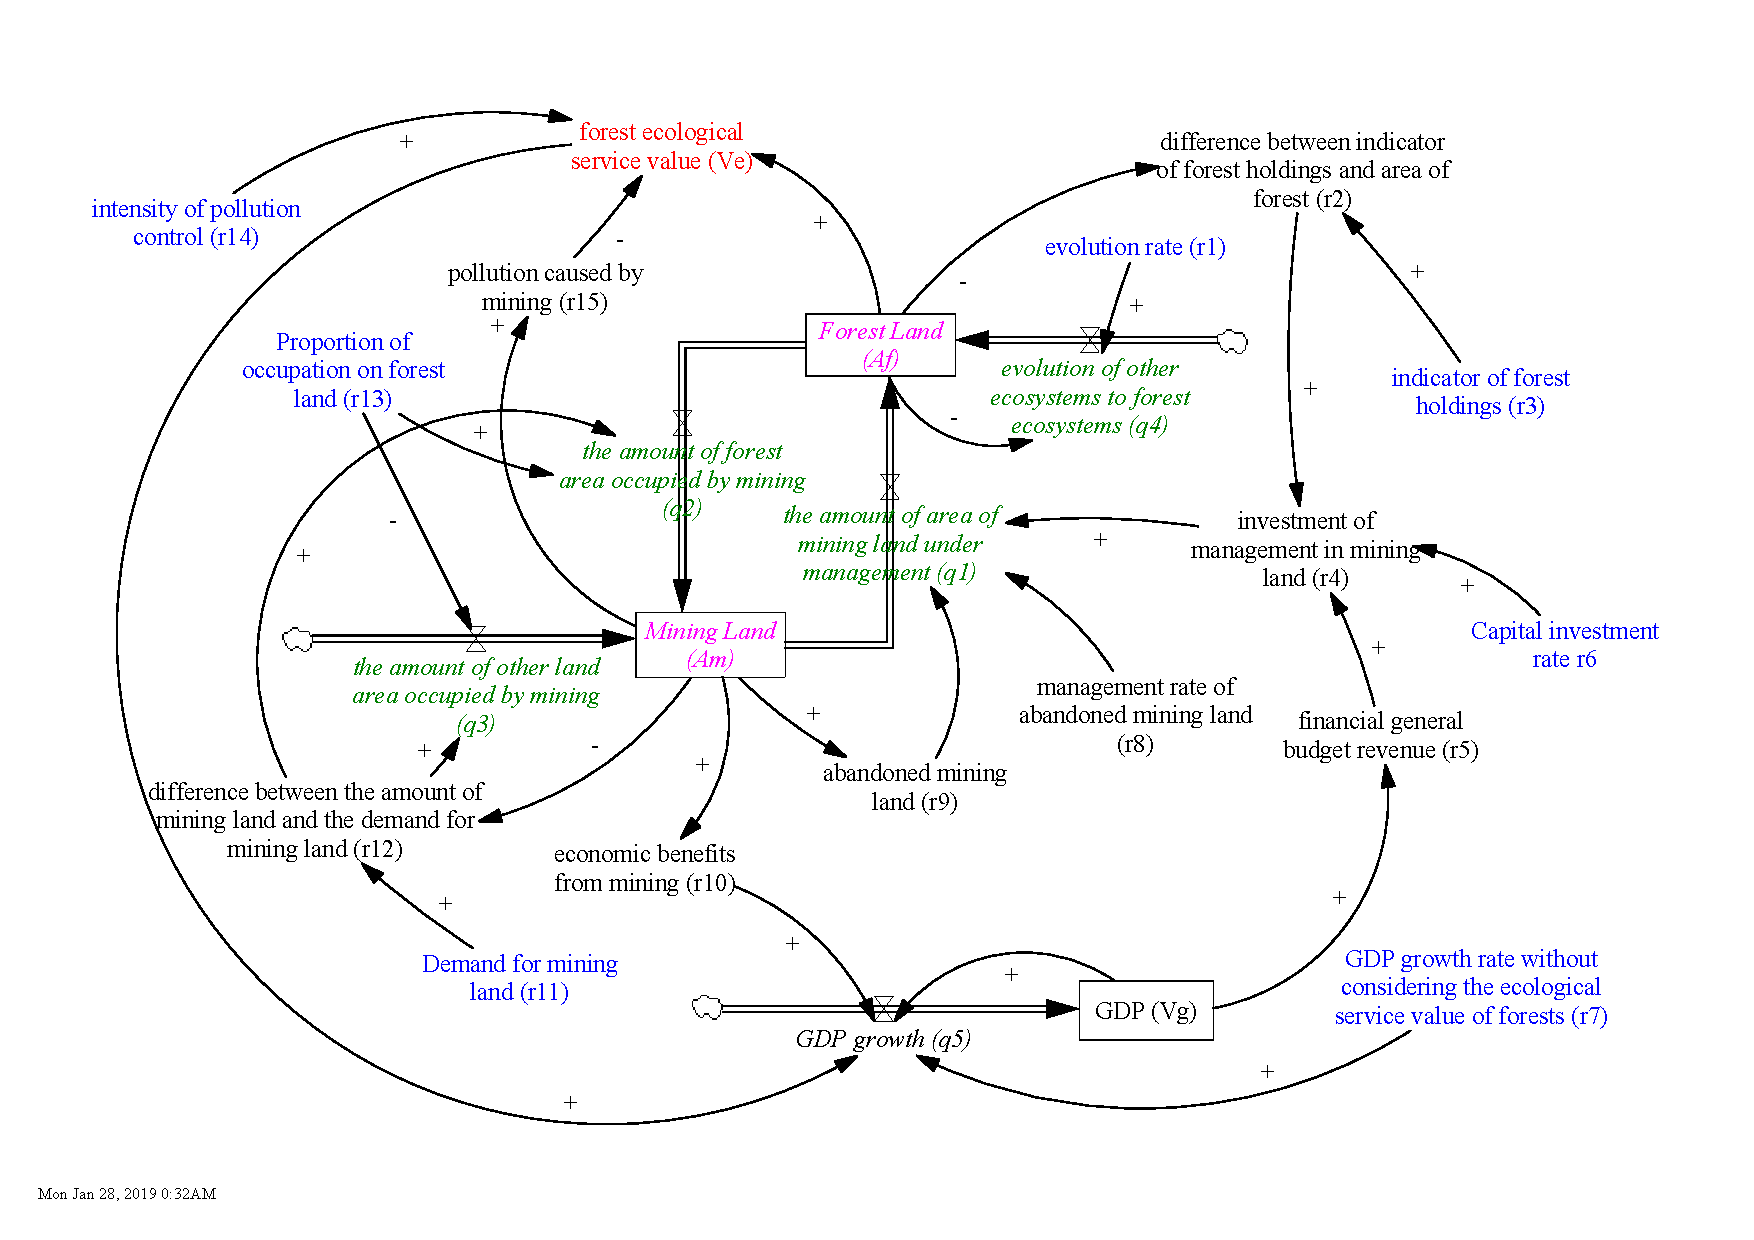
\includegraphics[width=\textwidth]{./pictures/dynamic.pdf}\\
  \caption{\small\heiti 森林生态系统土地面积变迁}\label{fig:dynamic}
\end{figure}

多图并列格式见图\,(\ref{fig:baifenbin})。

\begin{figure}[htbp]
\centering
\subfigure[\ce{CO2}]{
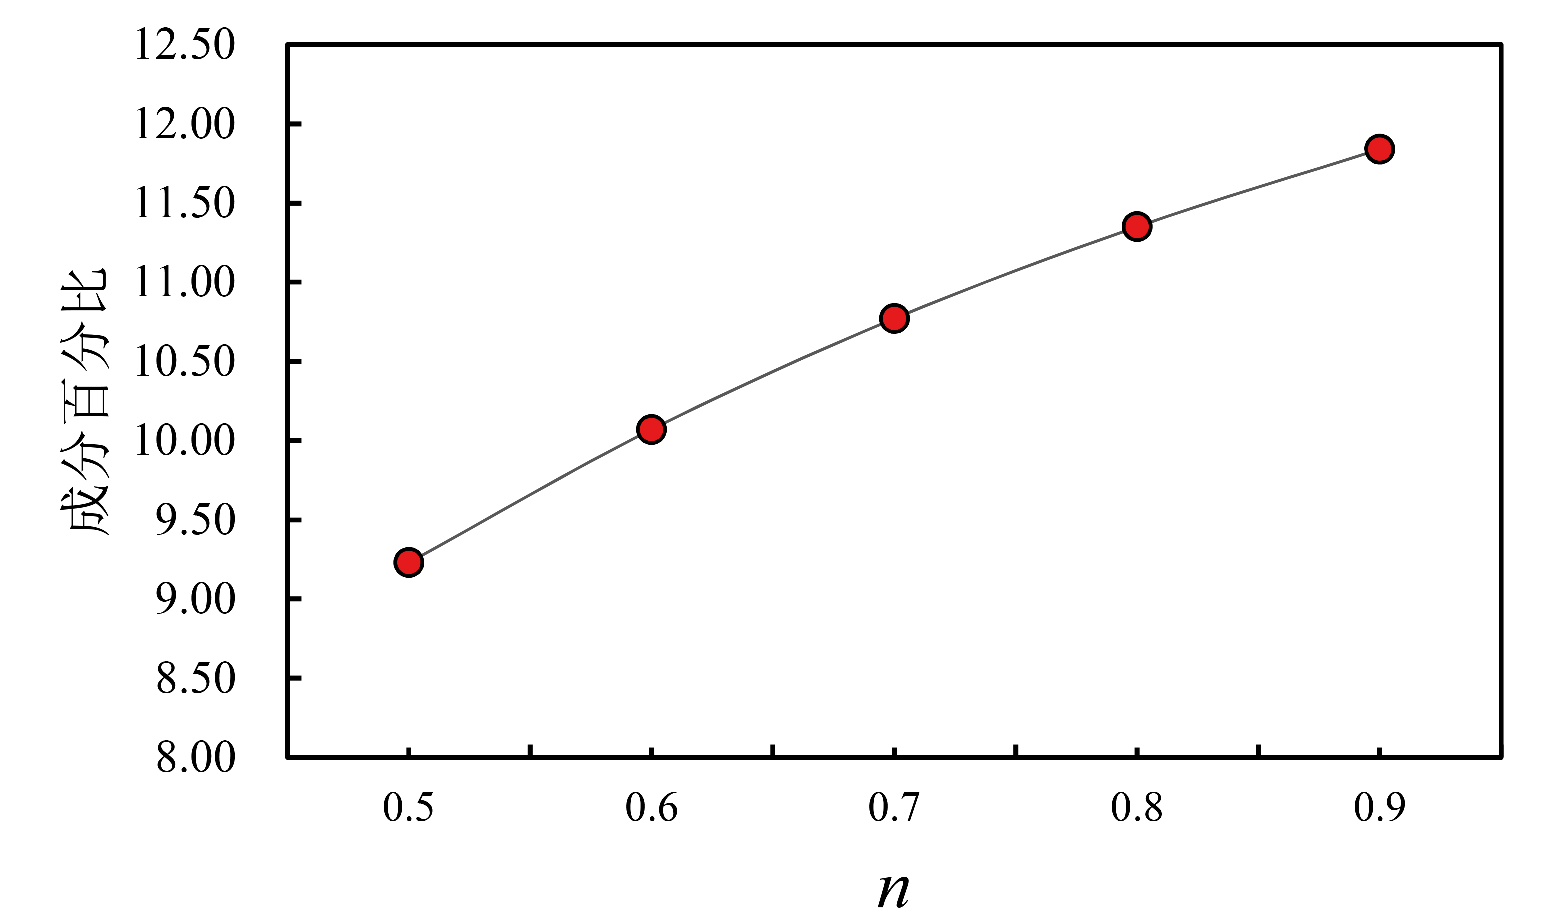
\includegraphics[width=0.46\textwidth]{./pictures/CO2.pdf}
}
\quad
\subfigure[\ce{CO}]{
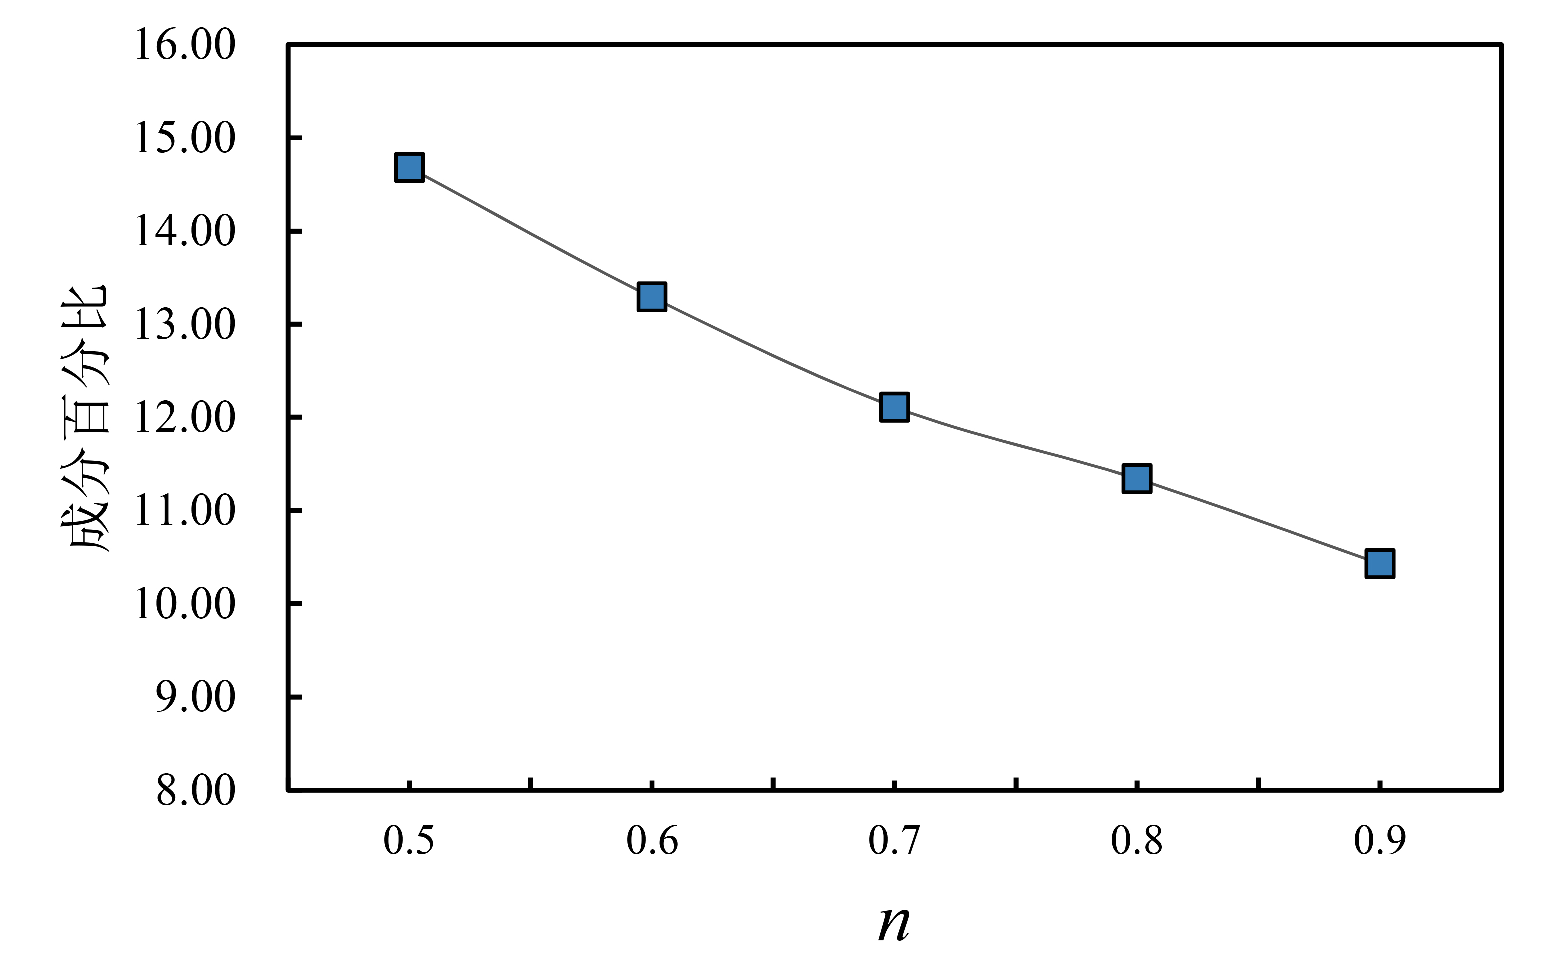
\includegraphics[width=0.46\textwidth]{./pictures/CO.pdf}
}
\quad
\subfigure[\ce{H2O}]{
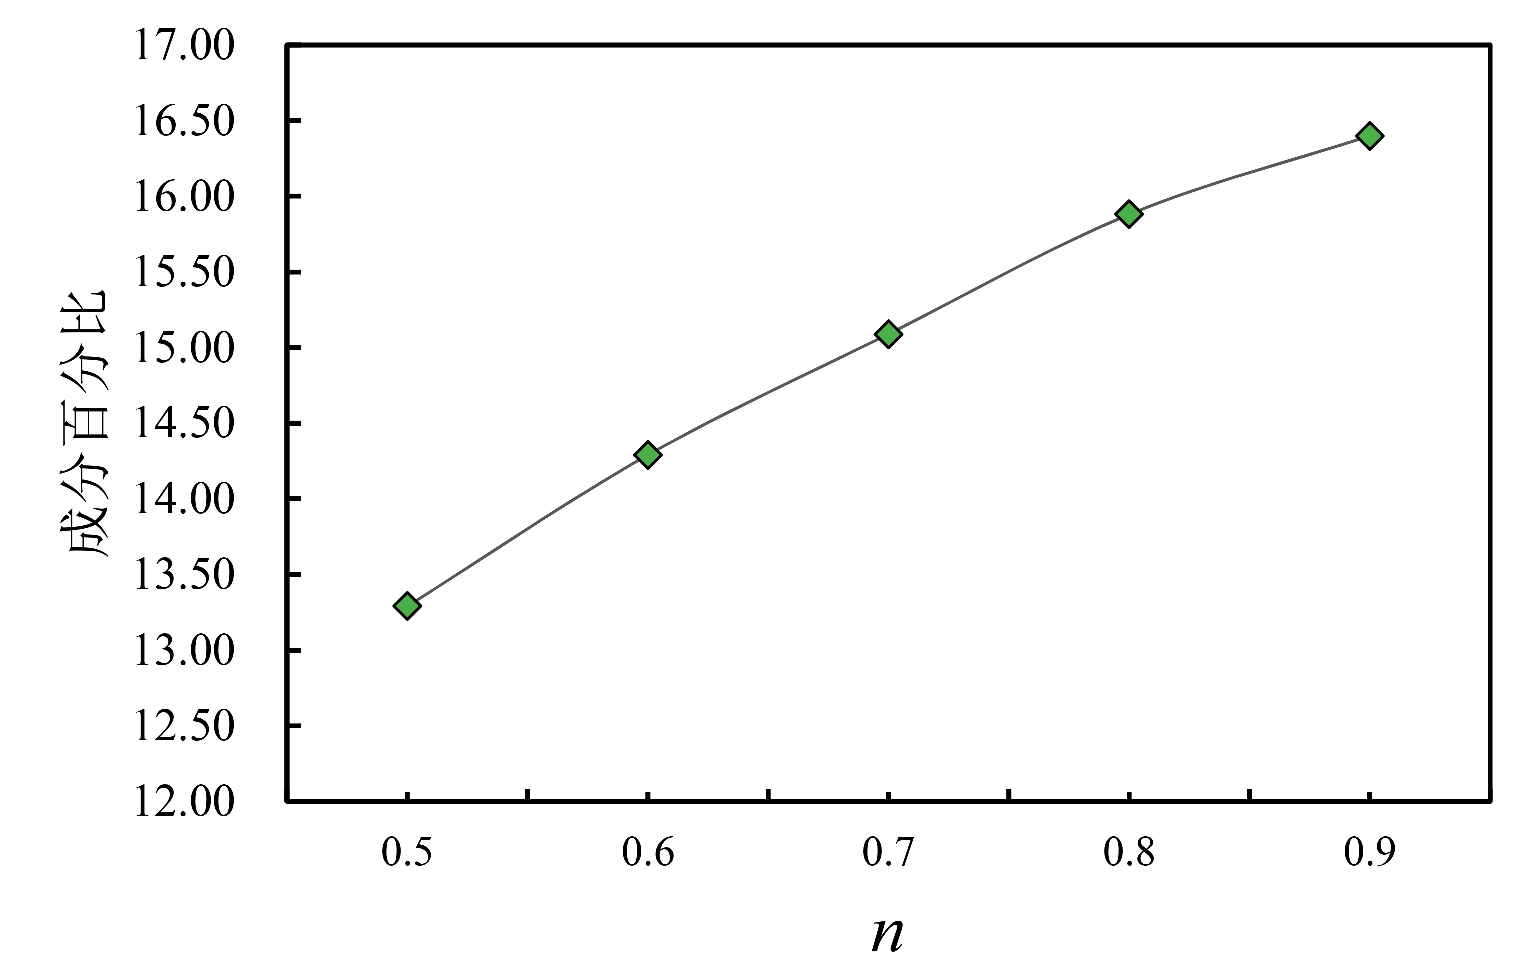
\includegraphics[width=0.46\textwidth]{./pictures/H2O.pdf}
}
\quad
\subfigure[\ce{H2}]{
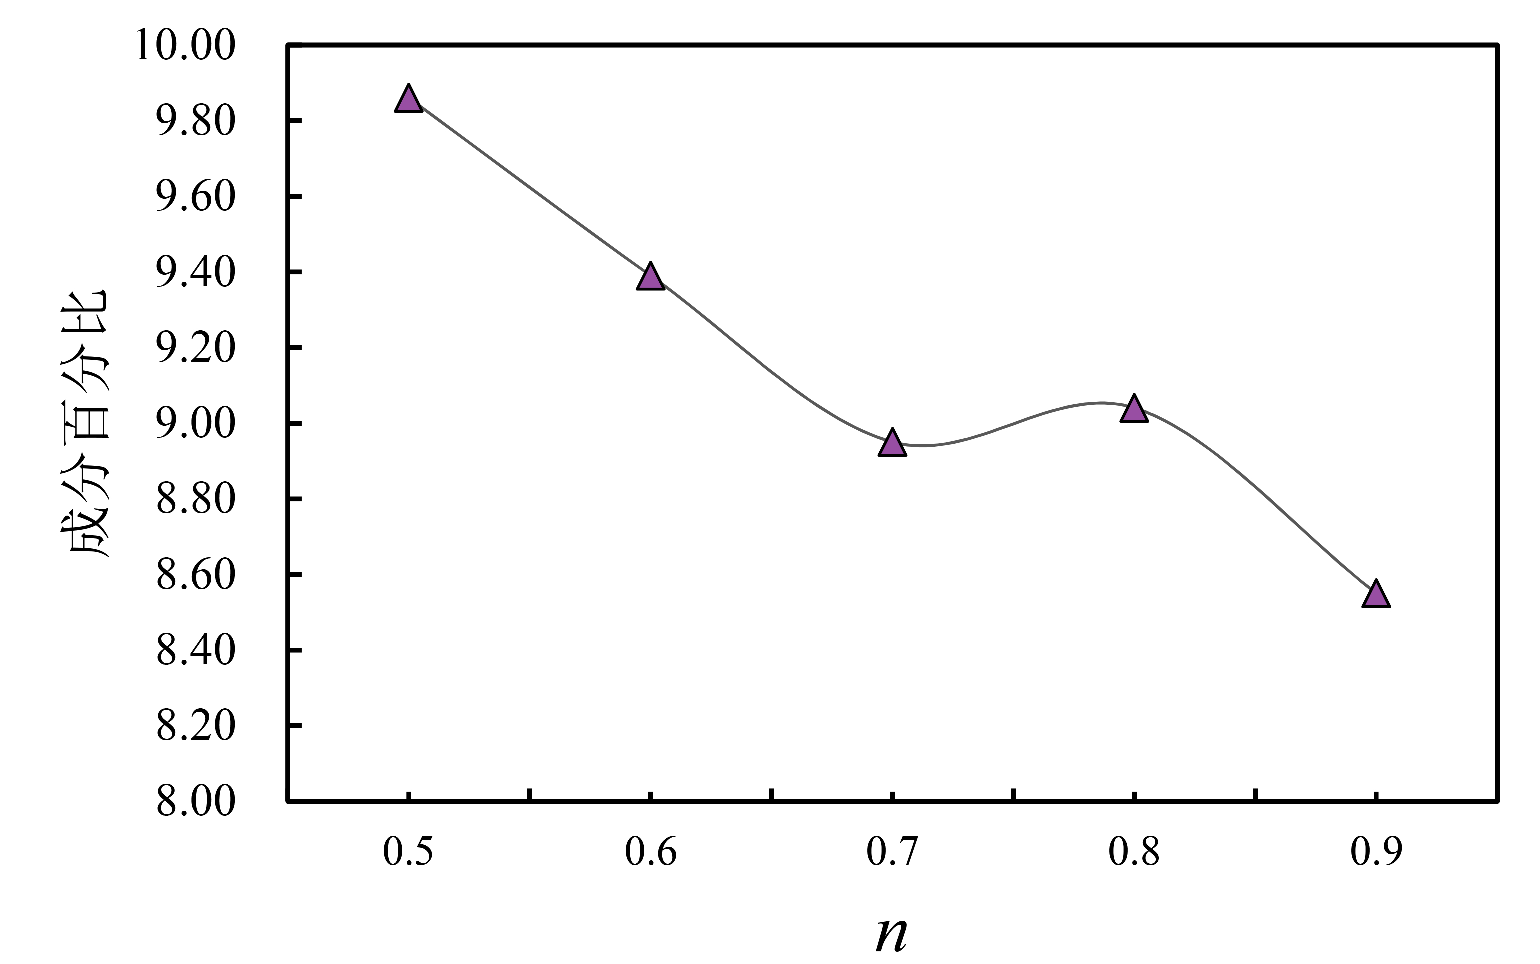
\includegraphics[width=0.46\textwidth]{./pictures/H2.pdf}
}
\quad
\subfigure[\ce{CH4}]{
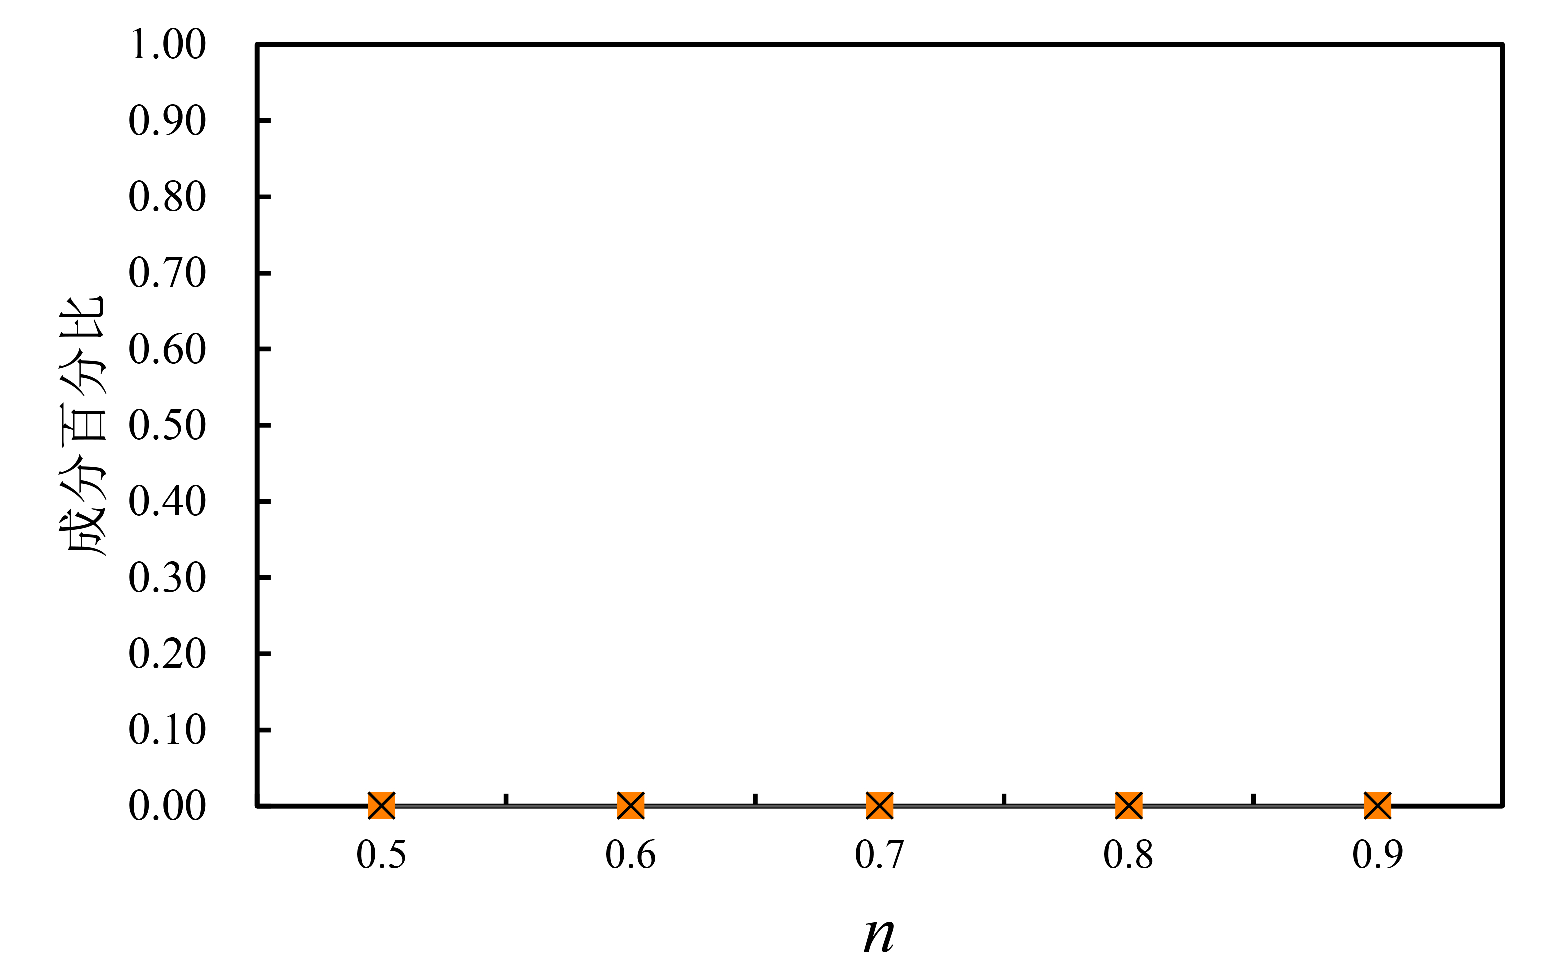
\includegraphics[width=0.46\textwidth]{./pictures/CH4.pdf}
}
\quad
\subfigure[\ce{N2}]{
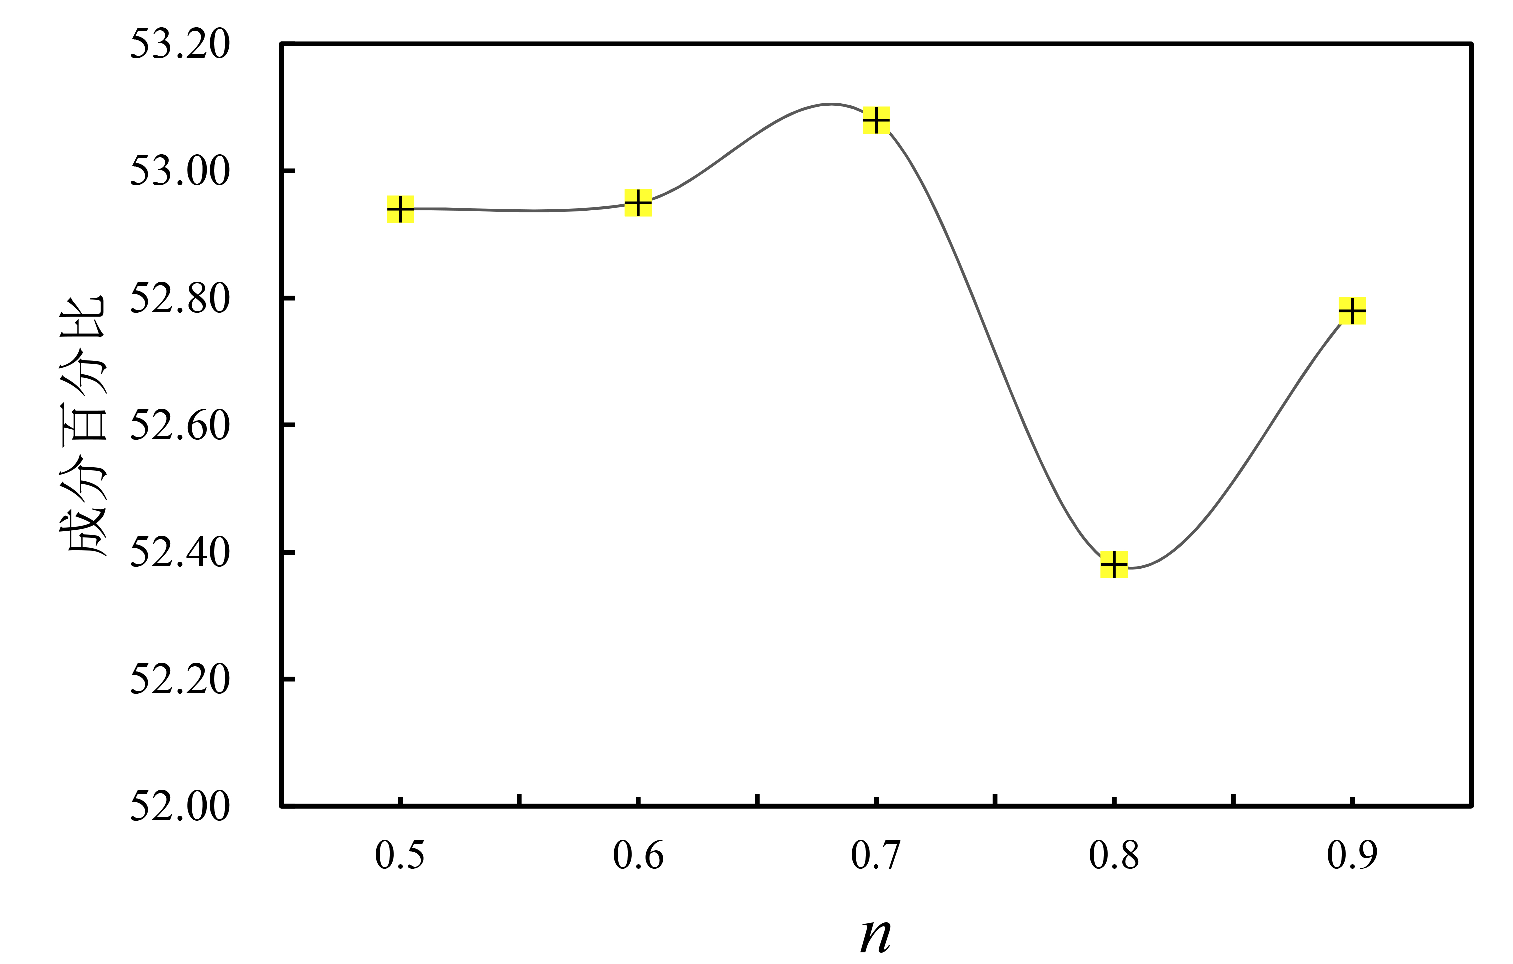
\includegraphics[width=0.46\textwidth]{./pictures/N2.pdf}
}
\caption{不完全燃烧产物成分百分比随$\,n\,$变化曲线图}\label{fig:baifenbin}
\end{figure}

\newpage\vspace*{-21.6pt}
\section{已知存在的问题}
本\LaTeX 模板中存在三个问题:

\begin{enumerate}[itemsep=0pt,parsep=0pt,label=\arabic*.]
  \item 目录中一级标题不是原Word文档中的“第1章\quad 概论”,而是“1\quad 概论”,但问题不大;
  \item 程序代码listings宏包与titletoc宏包疑似存在冲突(作者未找到具体起因),在排版程序代码时,可能报错:package inputenc error unicode char \verb"\u" 8 not set up use with latex,请谨慎使用listings宏包排版程序代码;
  \item 文献字体设置为楷体,而不是原Word文档中的楷体GB2312。
\end{enumerate}


\newpage
\phantomsection
\bibliography{./literature/thesis}
\nocite{*}
\appendix
\label{cod:matlab}
\newpage
\vspace*{-21.6pt}
\begin{center}
\zihao{3}\heiti
\phantomsection%设置“幻影标题”,解决额外插入目录(\addcontentsline)后总是引用到第一页的问题;
\addcontentsline{toc}{section}{附录}
附录
\end{center}

以下是布封投针求圆周率\,$\uppi$\,的Matlab的部分代码:
 %Matlab 代码格式设置
\definecolor{DarkGreen}{rgb}{0.0,0.4,0.0}
\lstloadlanguages{Matlab}
\lstset{language=Matlab,
	frame=shadowbox,                           % shadowbox framed
    rulesepcolor= \color{gray},%框的颜色
    breaklines=true,
	basicstyle=\small\ttfamily,
	keywordstyle=[1]\color{blue}\bfseries,  % primitive funs in bold blue
	keywordstyle=[2]\color{purple},         % args of funs in purple
	keywordstyle=[3]\color{blue}\underbar,  % user funs in blue with underbar
	stringstyle=\color{purple},             % strings in purple
	showstringspaces=false,
	identifierstyle=,
	commentstyle=\usefont{T1}{pcr}{m}{sl}\color{DarkGreen}\small,
	tabsize=4,
	% more standard MATLAB funcs
	morekeywords={sawtooth, square},
	% args of funcs
	morekeywords=[2]{on, off, interp},
	% user funcs
	morekeywords=[3]{FindESS, homework_example},
	morecomment=[l][\color{blue}]{...},     % line continuation (...) like blue comment
	numbers=left,
	numberstyle=\tiny\color{blue},
	firstnumber=1,
	stepnumber=1,
    escapeinside=``,
}

%插入 Matlab 脚本文件
\begin{lstlisting}[language=Matlab]
clear;clc;
n=2000;%`投针次数figure;`
axis([0,2,0,2]);
hold on;
plot([0,2],[0.5,0.5],'k','LineWidth',2);%`画y=0.5的直线`
plot([0,2],[1.5,1.5],'k','LineWidth',2);%`画y=1.5的直线`
x1=ones(1,n);y1=ones(1,n);%`投针中点坐标`
x2=ones(1,n);y2=ones(1,n);%`投针一端坐标`
x3=ones(1,n);y3=ones(1,n);%`投针另一端坐标`
jiaodu=ones(1,n);%`投针角度`
distant=ones(1,n);%`投针与最近直线的距离`
xianjiao=ones(1,n);%`投针与直线相交数`
for i=1:n %`开始投n次x1(1,i)=2*rand;`
    y1(1,i)=0.5+1*rand;
    jiaodu(1,i)=pi*rand;
    x2(1,i)=x1(1,i)-0.25*cos(jiaodu(1,i));
    y2(1,i)=y1(1,i)-0.25*sin(jiaodu(1,i));
    x3(1,i)=x1(1,i)+0.25*cos(jiaodu(1,i));
    y3(1,i)=y1(1,i)+0.25*sin(jiaodu(1,i));
    if(y1(1,i)<1)%`计算距离`
         distant(1,i)=y1(1,i)-0.5;
    else distant(1,i)=1.5-y1(1,i);
    end
end
n/sum(xianjiao)%`计算π`
\end{lstlisting}

\end{document}
